\documentclass[UTF8]{ctexart}

\usepackage{subfiles}  

%下面的语句, 引入你的头部设置文件
\usepackage{C:/phpStorm_proj/02_myself_ID_EGO/+100_latex_all_math_sel/myPreamble} 
%必须是绝对路径,才能让各个tex在单独编译时使用到

\title{文件名}


%---------------------------------


\begin{document}
	\tableofcontents % 生成目录
	\date{} % 若不写这句, 则默认也会渲染出日期, 所以我们要手动赋空值
	\maketitle  %这行代码, 让你前面的 title, author, date生效
	
		
	
	
	\part{ 事件的独立性}
	
	
	
	\section{(1)独立事件, (2)互斥(互不相容)事件, (3)对立事件 的区别 }	
	
	
	\begin{tabular}{|l|l|}
		\hline
		独立 &   $P(A \cap B)=P(A) \cdot P(B)$ \\	
		\hline
		互斥, 矛盾对立 &  $P(A \cap B)=0$, 并且 $P(A \cup B)=P(A) + P(B)$ \\	
		\hline
	\end{tabular} \\
	
	
	
	
	\subsection{独立事件 (一方对另一方的发生概率, 毫无影响) : \\ $P(A)×P(B)=P(A \cap B)$}
	
	(1)独立: \\
	- \textbf{是指 一个事件(A)的发生概率, 不受另一个事件(B)发生与否的影响.} 比如, 你抛两个骰子, 两个骰子的结果, 彼此互不影响. 它们可以点数不同, 也可以点数相同. \\
	- 即: $ P(A|B)=P(A)$.  ← 意思就是: 即使B发生的条件下, 来看A发生的情况, 其发生概率和A单独自己发生, 没有任何区别. 换言之, 有没有B先发生, 对A的发生概率毫无影响.\\
	- 若 A,B 是互相独立事件, 则:$ P(AB)=P(A) \cdot P(B) > 0$ \\
	- 反之, \textbf{独立事件判断标准就是:若 $P(A) \cdot P(B)=P(A \cap B)$, 则事件A和事件B, 为相互独立事件.}  \\
	
	
	\begin{myEnvSample}
		两个事件相互独立性判断的步骤: \\
		(1) 求出样本空间Ω 的样本点数 \\
		(2) 分别求出事件A、B、$A \cap B$的样本点数 \\
		(3) 分别求出P(A)、P(B)、P(AB) \\
		(4) 验证:P(A)×P(B)是否等于P(AB) \\
		(5) 如相等则为``独立性"事件, 反之为``非独立性"事件. \\
		
		换言之:只要满足P(A)×P(B)=P(AB),则AB 互为独立事件! \\
		
		例如: 抛两枚硬币: \\
		- 事件A: 抛出 一正一反 \\
		- 事件B: 抛出 至少一个正面 \\
		问:AB是否为互为独立事件? \\
		
		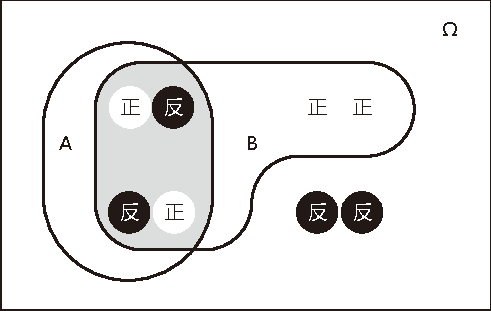
\includegraphics[width=0.6\textwidth]{/0114.pdf} \\
		
		第1步:求样本空间样本点数,Ω \{(正,正),(正,反),(反,正),(反,反)\} = 4个样本点 \\
		
		第2步:求A、B、$A \cap B$的样本点数 : \\
		- A抛出:一正一反,即A \{ (正,反),(反,正) \} =2个样本点数 \\
		- B抛出:至少一个正面,即B \{ (正,反),(反,正),(正,正) \} =3个样本点数 \\
		- $A \cap B$:一正一反,即AB \{ (正,反),(反,正) \} =2个样本点数 \\
		
		第3步:求出P(A)、P(B)、P(AB): \\
		- P(A)=2/4 \\
		- P(B)=3/4 \\
		- P(AB)=2/4 \\
		
		
		第4步:看 P(A)×P(B) 是否等于P(AB)? \\
		P(A)×P(B)=(2/4)×(3/4)=3/8,不等于P(AB)=2/4 \\
		所以, 事件A与事件B不是相互独立事件.
		
	\end{myEnvSample}
	
	
	
	- 多个事件彼此独立 : 若 A,B,C 互相独立, 则有: 
	\begin{align*}  % 支持每行编号. 若不需要编号, 就用 align*环境
		& P(AB)=P(A)\cdot P(B)\\
		& P(BC)=P(B)\cdot P(C)\\
		& P(AC)=P(A)\cdot P(C)\\
		& P(ABC)=P(A)\cdot P(B)\cdot P(C) 
	\end{align*}
	
	
	
	~\\
	\hrule
	~\\
	
	
	\subsection{互斥事件 (曹操,刘备,是``互拆"事件关系. 但它们的并集不构成天下的Ω全集, 还有其他竞争诸侯存在) : $P(A)+P(B)=P(A \cup B)$}
	
	(2)互斥(互不相容), 彼此矛盾对立: \\
	- \textbf{它指的是: 两个事件不可能同时发生} (至多只有一个发生. 它们可能都不发生, 但不会同时发生). 或 两个结果不可能同时出现. \\
	-  是指两个事件没有交集. \\
	- 从集合的角度看, 几个事件彼此``互斥", 就是指各个事件所含的基本事件组成的集合, 彼此互不相交. \\
	- \textbf{即 $ AB=\varPhi $ 空集.  有你没我, 有我没你.} AB同时发生的可能性为0. \\
	- 比如,一个人的性别不是男就是女, 不可能同时既是男又是女. \\
	
	- 于是可以得到:若AB为互斥事件,A和B发生的概率 P($A \cup B$)=P(A)+P(B) \\
	- 反过来, 就是: 若要证明 事件A和事件B为互斥事件,则只需证明 P(A)+P(B)=P(A+B) \\
	
	
	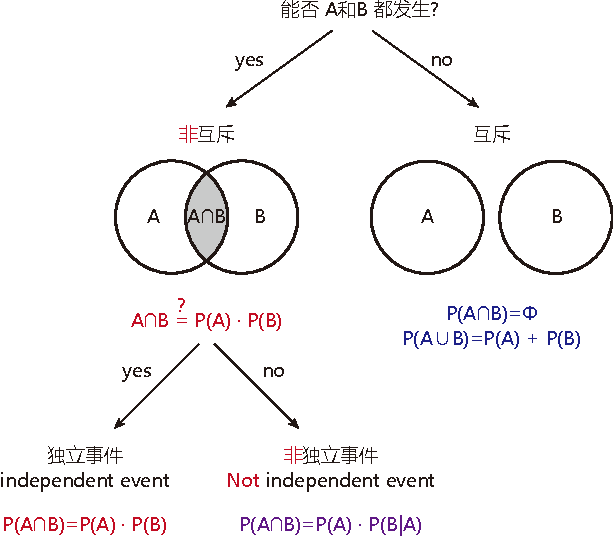
\includegraphics[width=0.7\textwidth]{/0113.pdf} \\
	
	
	``独立"与``互斥"不会同时成立. \\
	
	
	
	
	注意区别:	\\
	→ 事件A的``条件概率" $P(A|B)$ :  \\
	事件B的发生, 改变了事件A发生的概率, 也即事件B对事件A有某种``影响”. \\
	
	→ 事件A的``无前提条件的概率" $P(A)$ : 这里, 事件B的发生, 对事件A的发生毫无影响,即$ P(A|B)=P(A)$.  \\
	由此又可推出 $ P(B|A)=P(B)$, 即事件A发生对B也无影响. 可见独立性是相互的.  \\
	
	
	\begin{myEnvSample}
		已知: $P(A \cup B)=0.9, P(A)=0.4$, 问: \\
		
		- 当A, B 互斥时, P(B)=? \\
		A, B互斥, 即说明 AB的交集=Φ,  即 P(AB)=0. \\
		因为 $\underset{=0.9}{\underbrace{P(A+B)}}=\underset{=0.4}{\underbrace{P(A)}}+P(B)-\underset{=0}{\underbrace{P(AB)}}$ \\
		所以 $P(B)=0.9-0.4-0=0.5$ \\
		
		
		
		- 当A, B 独立时, P(B)=? \\
		两个事件彼此独立, 则有公式: $P(AB) = P(A) \cdot P(B)$ \\
		但注意: 这里的 P(AB) 不能直接搬用上面的值0. 因为这里的A,B是独立事件, 而非上面的互斥事件.  
		\begin{align*}  % 支持每行编号. 若不需要编号, 就用 align*环境
			&\underset{=0.9}{\underbrace{P(A+B)}}=\underset{=0.4}{\underbrace{P(A)}}+P(B)-\underset{=P(A)\cdot P(B)}{\underbrace{P(AB)}}\\
			&\text{即:\ }0.9=0.4+P(B)-0.4\cdot P(B)\\
			&0.9-0.4=(1-0.4)\cdot P(B)\\
			&P(B)=\frac{0.5}{0.6}=\frac{5}{6}=0.833333
		\end{align*}
		
		
	\end{myEnvSample}
	
	
	~\\
	\hrule
	~\\
	
	
	\subsection{对立事件 (平分天下的刘邦,项羽, 是``对立"事件关系) : \\ P(A+B)=P(A)+P(B)=1=Ω }
	
	- 通俗的说:所有可能的结果非黑即白, 并且他们的并集能组成全集Ω, 就叫对立事件! \\
	如, 一个婴儿出生,要么是男孩,要么是女孩. \\
	争夺天下, 要么成王, 要么败寇. \\
	一道选择题,只有2个选项A和B,要么选A,要么选B. \\
	
	
	- 若AB为对立事件,且A+B=Ω,则AB互为对立事件.  \\
	反过来说, 即: 若AB为对立事件,A和B发生的概率 P(A+B)=P(A)+P(B)=1 \\
	还可以得到:若AB为对立事件,P(A)=1-P(B) \\
	
	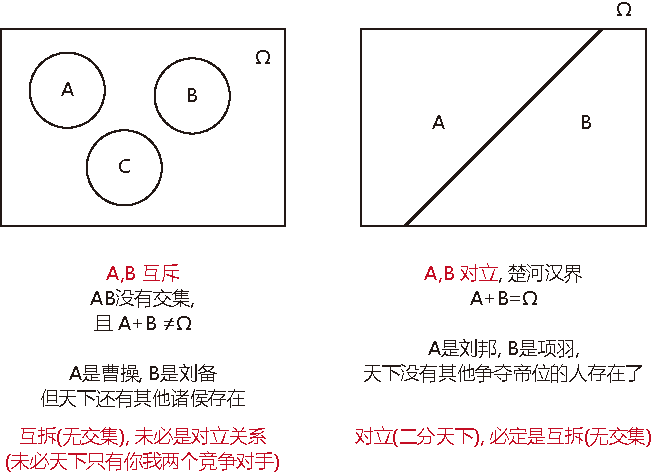
\includegraphics[width=0.75\textwidth]{/0115.pdf} \\
	
	
	
	- 对立事件,必定是互斥事件,但互斥事件,未必是对立事件. \\
	所以可以说:互斥事件,是对立事件的前提条件(必要条件)
	
	
	
	~\\
	\hrule
	~\\
	
	\section{A,B 是两个相互独立的事件, 则有: $P(AB)= P(A) \cdot P(B)$}
	
	即, 事件相互独立: 就是指一个事件发生,不会影响另一个事件的发生或不发生. 两个事件没有相关性,相关系数为0. \\
	从数学上定义, 就是$ P(AB)=P(A) \cdot P(B)$ \\
	即: 两个相互独立的事件A和B 都发生的概率, 等于每个事件发生的概率的积. (即等于``分步骤法".) \\
	
	另外:  ``Φ 和 Ω" 与``任意事件A" 都独立. \\
	
	
	\begin{myEnvSample}
		甲乙丙三人投篮(显然这三个人的命中率是独立事件, 彼此互不影响), 命中率分别是: \\
		- 甲投中(A事件) : P(A)=0.7.  则甲没投中的概率就是 $P(\overline{A}) =1- P(A) =0.3$ \\
		- 乙投中(B事件) : P(B)=0.8.  乙没投中就是 $P(\overline{B})=0.2$\\
		- 丙投中(C事件) : P(C)=0.75.  丙没投中就是 $P(\overline{C})=0.25$\\
		
		问: \\
		→ 他们各投一次, 恰有一人投中的概率: 		
		\begin{align*}  % 支持每行编号. 若不需要编号, 就用 align*环境
			&=P\left( A\overline{B}\overline{C}\cup \overline{A}B\overline{C}\cup \overline{A}\overline{B}C \right)\\
			&=P\left( A\overline{B}\overline{C} \right) +P\left( \overline{A}B\overline{C} \right) +P\left( \overline{A}\overline{B}C \right) \\
			&  ←\ \text{因为}ABC\text{是独立事件,所以它们乘积的概率,就等于各自概率的乘积}\\
			&=\underset{}{\underbrace{P\left( A \right) \cdot P\left( \overline{B} \right) \cdot P\left( \overline{C} \right) }}+\underset{}{\underbrace{P\left( \overline{A} \right) \cdot P\left( B \right) \cdot P\left( \overline{C} \right) }}+\underset{}{\underbrace{P\left( \overline{A} \right) \cdot P\left( \overline{B} \right) \cdot P\left( C \right) }}
		\end{align*}
		
		→ 三人全部投中的概率: $P(ABC)=P(A)\cdot P(B)\cdot P(C)$ \\
		
		→ 至少有一人投中的概率 (即 >= 1人, 就是把``0人投中"排除出去后,剩下的全部) : \\
		$=1-\underset{\text{所有人全没投中}}{\underbrace{P(\overline{A}\overline{B}\overline{C})}}=1-\underset{ABC\text{是独立事件,所以它们乘积后的概率,就等于各自概率的乘积}}{\underbrace{P\left( \overline{A} \right) \cdot P\left( \overline{B} \right) \cdot P\left( \overline{C} \right) }}	$	
	\end{myEnvSample}
	
	\vspace{1em} 
	
	
	\begin{myEnvSample}
		破译某密码, 如果仅靠一个人去破译, 成功概率是 0.6 (即60\%). \\
		问: 如果想将成功率提高到99\%, 至少需要多少人来一起破译? \\
		
		显然, 每个人的破译成功率, 彼此间毫无影响, 是``独立事件"关系的. \\
		我们先设: \\
		- $A_i$ : 表示是第i个人破译出了密码. \\
		- B : 表示破译成功. 即 $B=\bigcup_{i=1}^n{A_i}$, ← 也就是说 : 只要一堆A里面任何一个人成功了, 就相当于整个团队完成了任务. (这里就用了并集). \\
		
		我们倒过来想: 成功概率, 就等于1减去``大家都没成功的概率". 即: 
		
		\begin{align*}  % 支持每行编号. 若不需要编号, 就用 align*环境
			&P(B)=1-\underset{\text{连乘后的概率}}{\underbrace{P\left( \bigcap_{i=1}^n{\overline{A_i}} \right) }}\ ←\ 1\text{减去}“\text{每一个人都失败了,即失败交集的概率}”\\
			&=1-\prod_{i=1}^n{P\left( \overline{A_i} \right)}\ ←\ “\text{连乘}”\text{后的概率,就等于概率后的乘积}\\
			&=1-0.4^n\ ←\ \text{每一个人失败的概率}=1-\text{成功率}0.6=0.4.\ \text{然后一共有}n\text{个人在做破解工作}. 
		\end{align*}
		
		上面, $0.4^n$ 就是 n个人都失败 的概率. \\
		
		即我们要让 : 
		\begin{align*}  % 支持每行编号. 若不需要编号, 就用 align*环境
			&P\left( B \right) \ge 0.99\\
			&1-0.4^n\ge 0.99\\
			&n \approx 5.026  
		\end{align*}
		
		即, 至少需要6个人才行.
	\end{myEnvSample}
	
	
	%\vspace{1em} 
	
	
	%
	%\begin{myEnvSample}
	%已知: $
	%\left\{ \begin{array}{l}
		%	0<P\left( A \right) <1\\
		%	0<P\left( B \right) <1\\
		%	P\left( A|B \right) +P\left( \overline{A}\ |\overline{B} \right) =1\ \ (1)\\
		%\end{array} \right. 
		%$ \\
		%证明 A,B 是独立事件. \\
		%
		%首先, 我们知道 这个式子永远成立: $
		%\boxed{
			%P(A|\overline{B})+P\left( \overline{A}\ |\overline{B} \right) =1} \ (2)$
		%\end{myEnvSample}
		
		
		
		
		
		\section{若A,B是互相独立的事件, 则有: (1) A与$ \overline{B}$ 独立; (2) $ \overline{A}$ 与B独立; (3) $ \overline{A}$ 与 $ \overline{B}$ 独立}
		
		既然A,B 是相互独立的事件了, 彼此发生或不发生, 对另一方毫无影响. 所以, 我上不上岸 (A 或 $\overline{A}$), 和你结不结婚(B 或 $\overline{B}$)毫无影响. 
		
		
		
		\section{若 $P(A)=0$ 或 $P(A)=1$, 则 A与``任意事件"都互相独立.}	
		
		
	
	
	
	
	
	
\end{document}